\newpage
\subsection{Caso d'uso UC14: Amministrazione Applicazione Web}
\label{UC14}
\begin{figure}[ht]
	\centering
	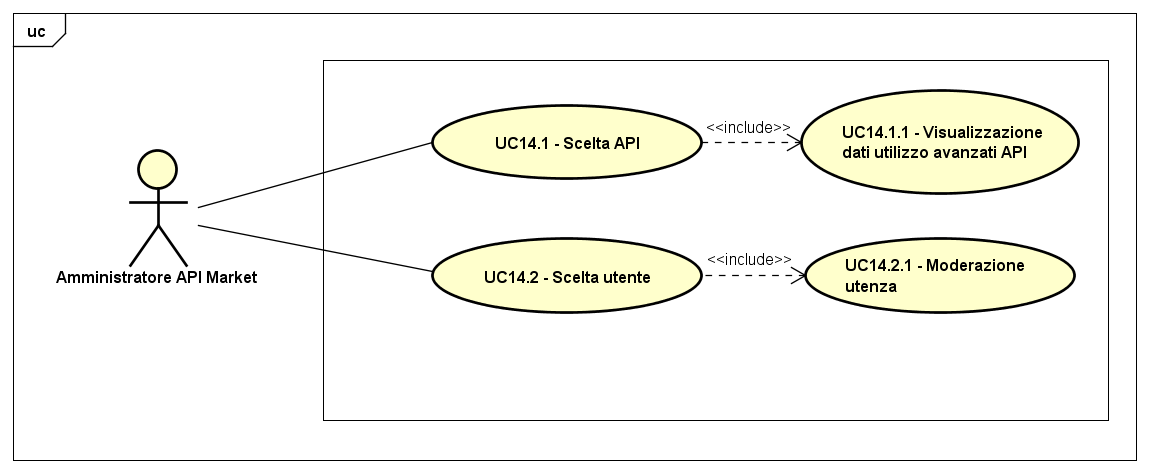
\includegraphics[scale=0.45]{UML/UC14.png}
	\caption{UC13: Visualizzazione Dati Utilizzo API}
\end{figure}

\renewcommand*{\arraystretch}{1.6}
\begin{longtable}{ l | p{11cm}}
	\hline
	\rowcolor{Gray}
	\multicolumn{2}{c}{UC14: Amministrazione Applicazione Web} \\
	\hline
	\textbf{Attori} &Utente Autenticato, Amministratore APIMarket \\
	\textbf{Descrizione} &l''attore visualizza i dati dell'utilizzo delle API in APIMarket \\
	\textbf{Pre-Condizioni} &   l'attore ha scelto di visualizzare i dati dell'utilizzo delle API in APIMarket\\
	\textbf{Post-Condizioni}& l'attore ha visualizzato i dati dell'utilizzo delle API in APIMarket\\
	\textbf{Scenario Principale} & \begin{enumerate*}[label=(\arabic*.),itemjoin={\newline}]
		\item L'attore può visualizzare il numero di utenti che hanno acquistato una API (UC13.1)
		\item L'attore può registrare l'interfaccia della propria nuova API (UC13.2)
	\end{enumerate*}\\
\end{longtable}


